% don't remove the folling lines, and edit the defintion of \main if needed
\documentclass[../report.tex]{subfiles}
\providecommand{\main}{..}
\IfEq{\jobname}{\currfilebase}{\AtEndDocument{\biblio}}{}
% until here

\begin{document}

\section{Quarkonia}

\subsection{Introduction (Main contributor: Ralf Rapp)}

\subsection{Charmonia in PbPb collisions (Main contributor: Anton Andronic)}


\begin{figure}

\begin{center}
 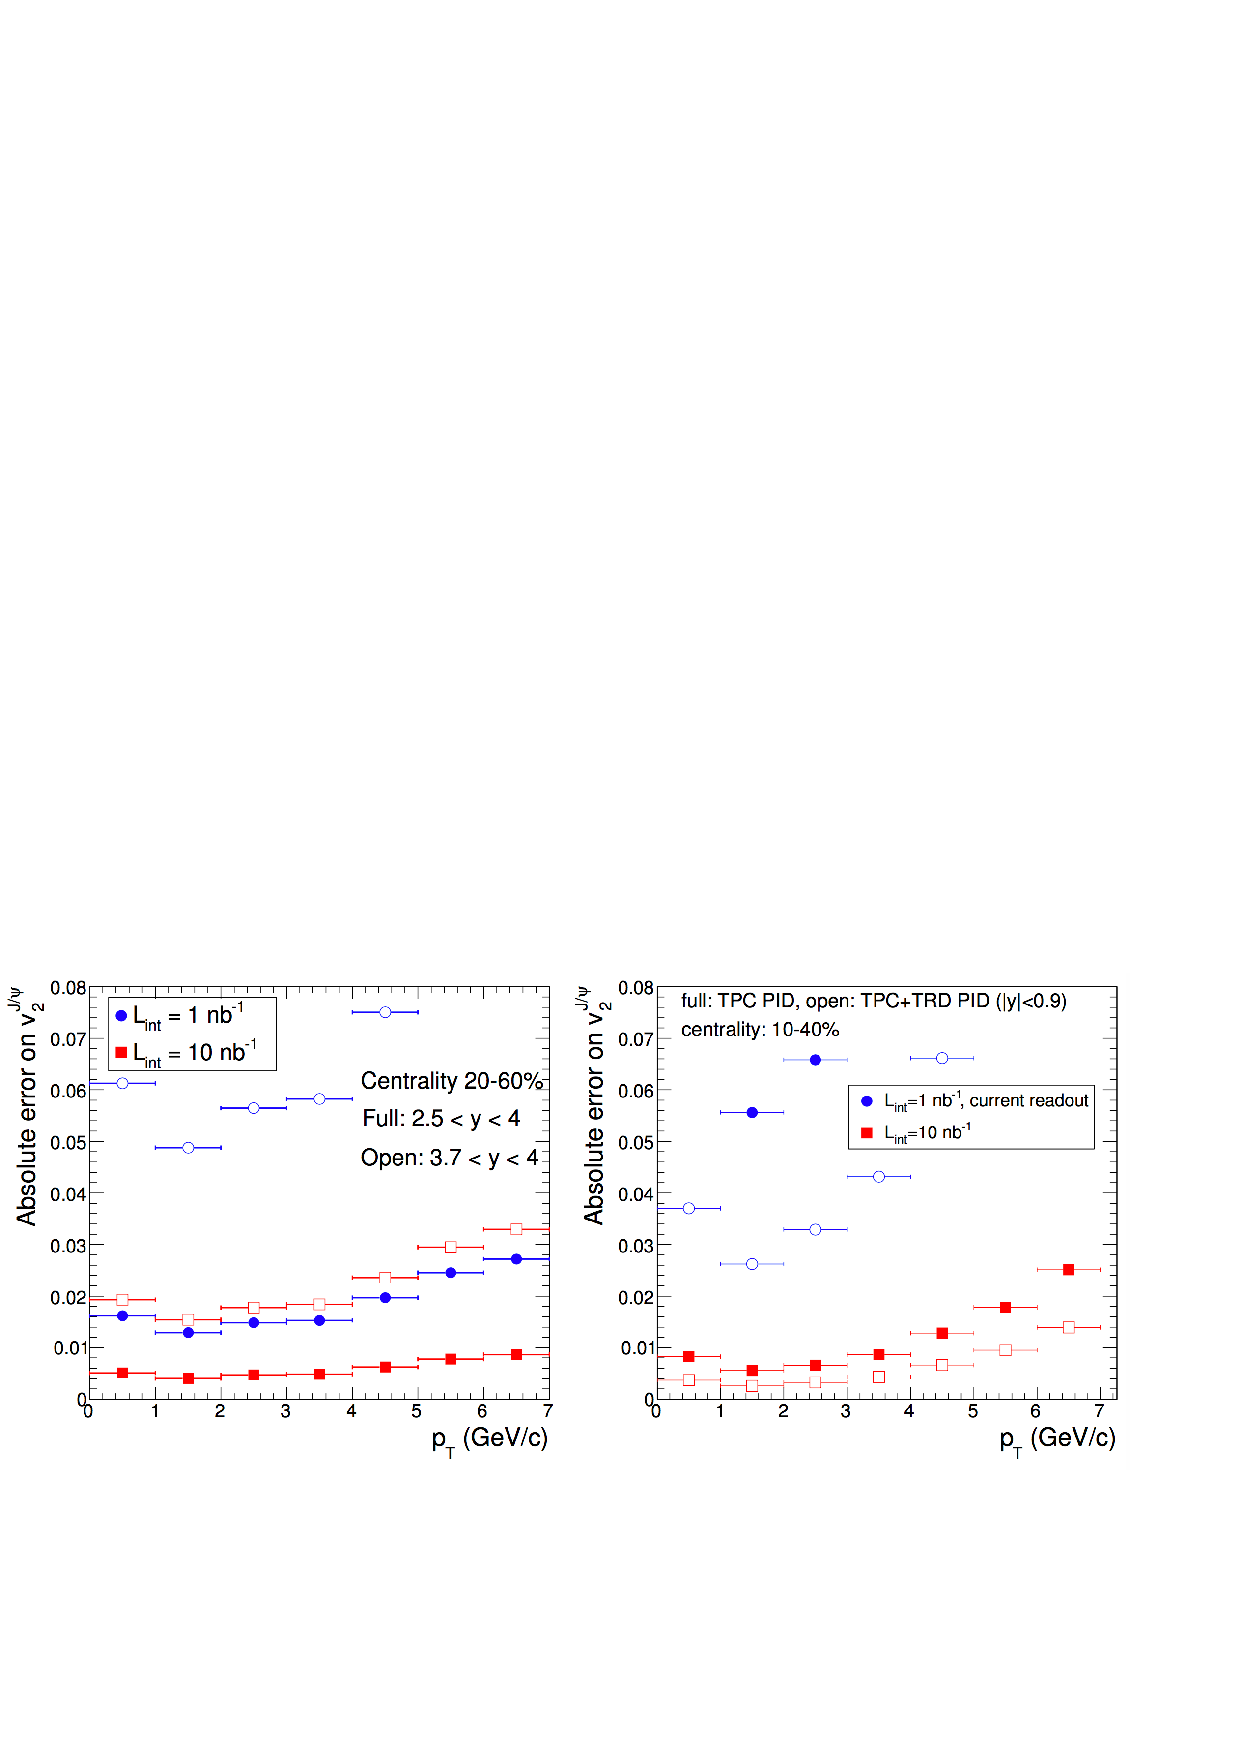
\includegraphics[width=0.66\textwidth]{fig/alice/alice_jpsi_v2_projected.pdf}
 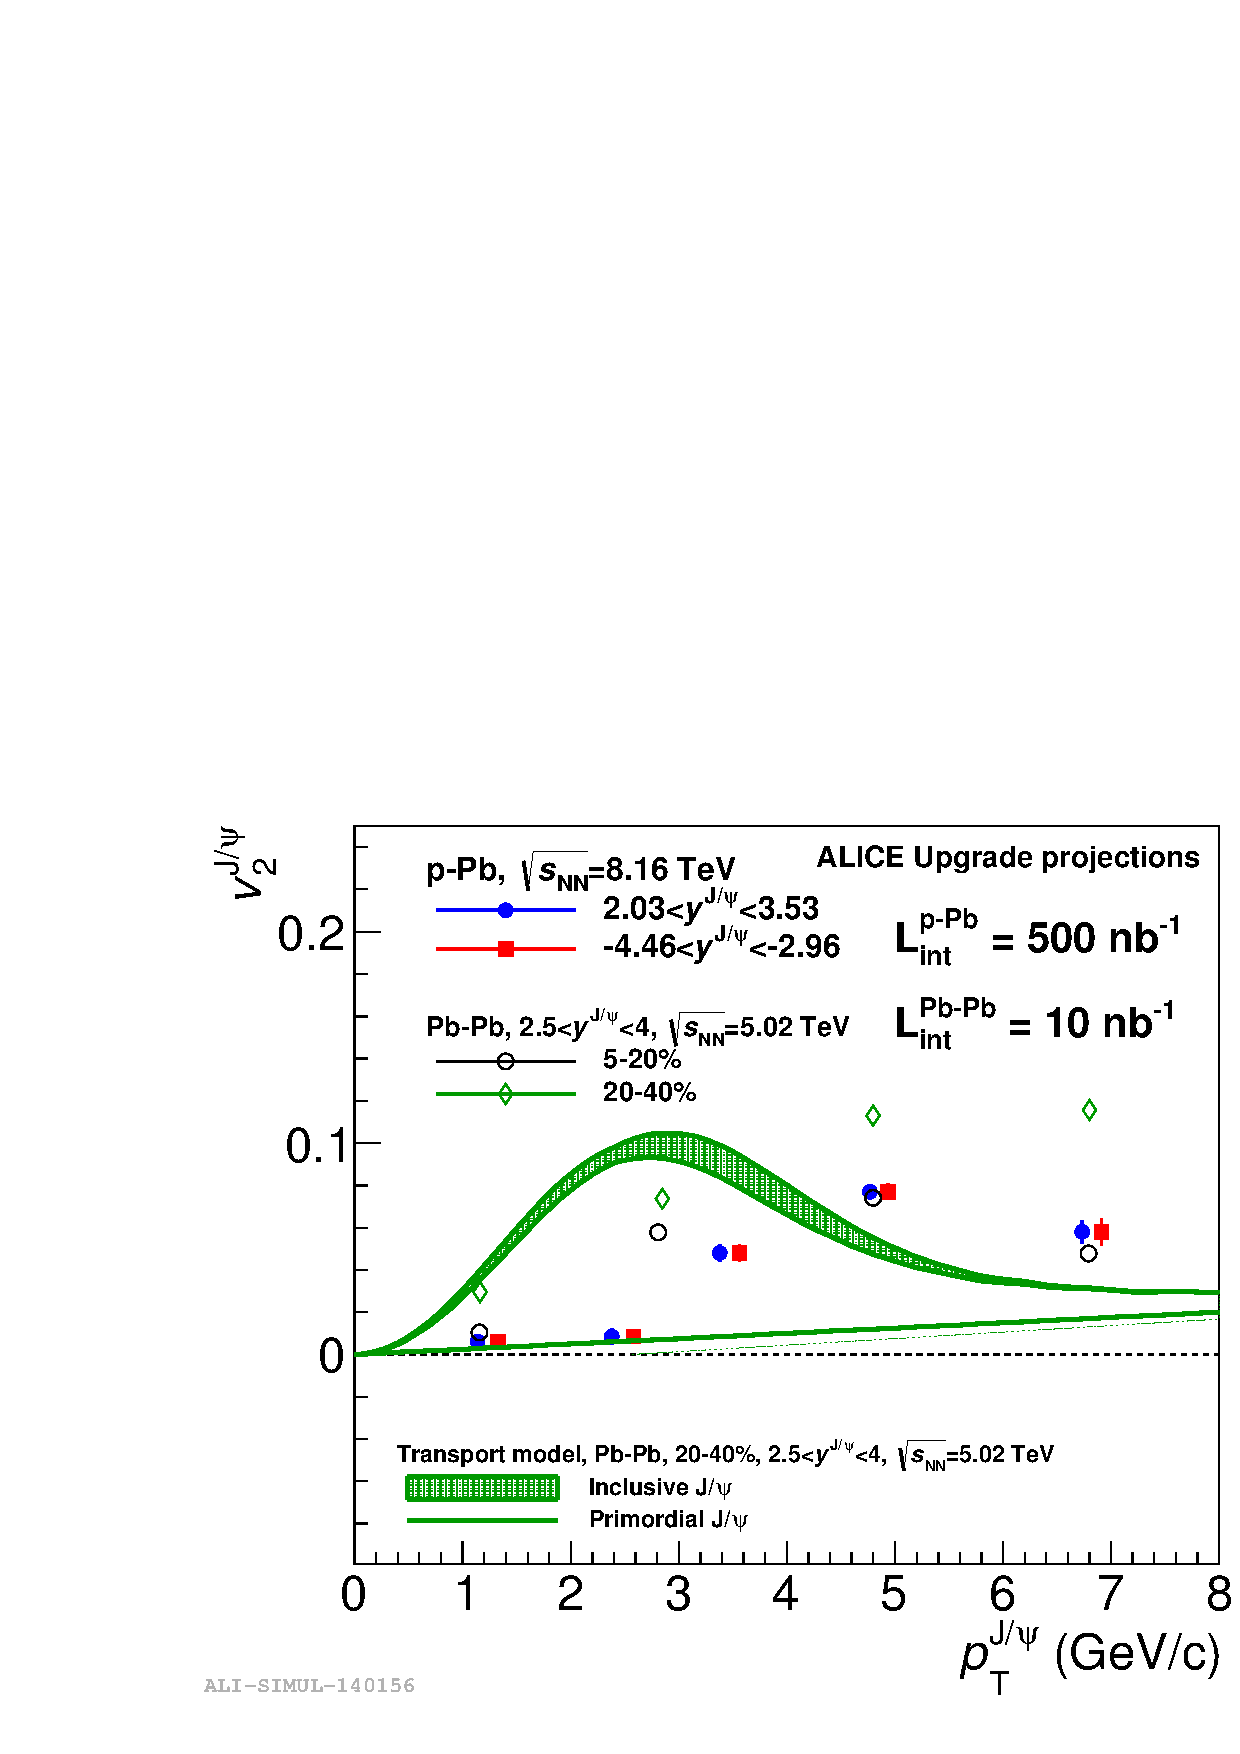
\includegraphics[width=0.32\textwidth]{fig/alice/alice_jpsi_v2_projected2.pdf}
\end{center}

 \caption{prompt J/psi v2 vs pT, for 30--50\%: $|y|<0.9$, $1.6<|y|<2.4$, $2.5<|y|<4$~\cite{Abelev:1475243,CERN-LHCC-2013-014}}
\end{figure}

\begin{figure}
\begin{center}
 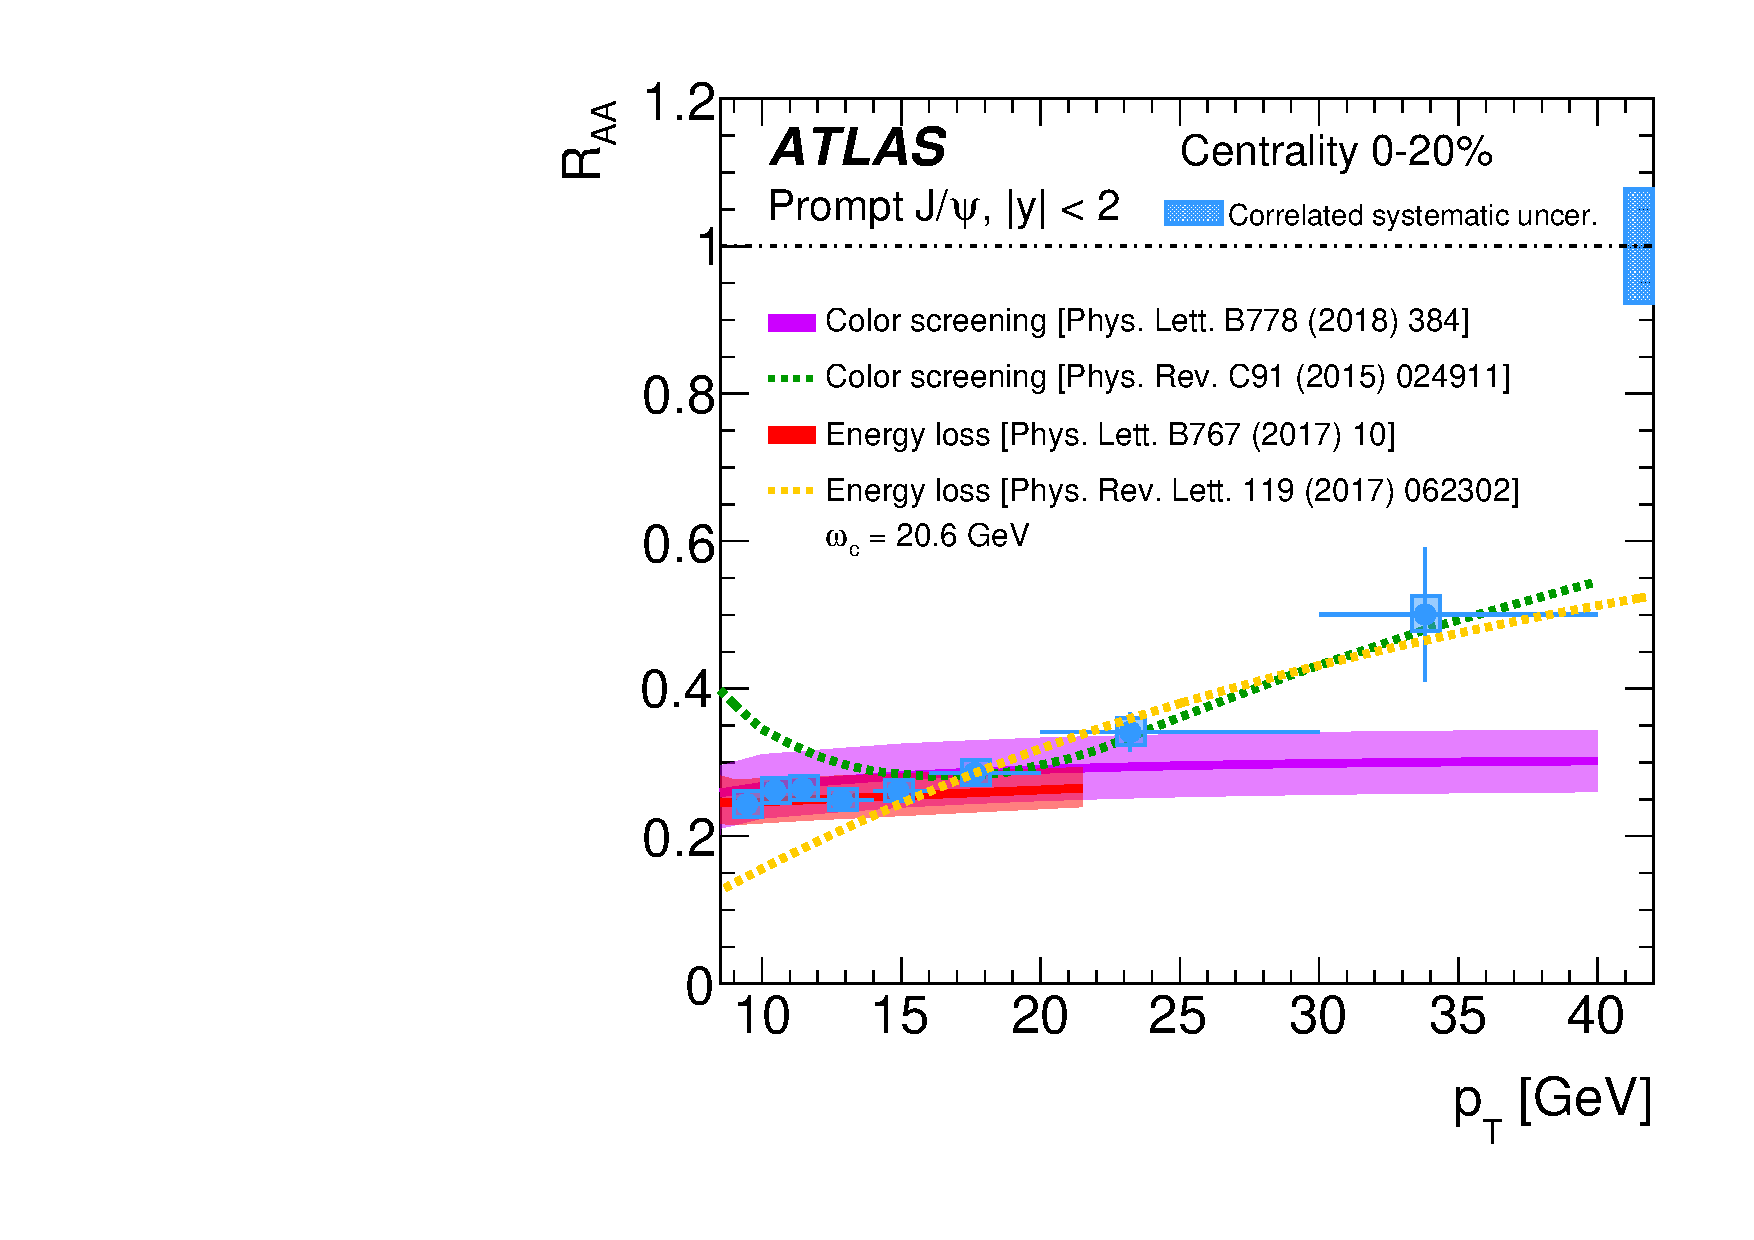
\includegraphics[width=0.5\textwidth]{fig/atlas/atlas_promptjpsi_models}
\end{center}

 \caption{prompt J/psi RAA vs Pt ($|y|<2.4$) at high pT~\cite{Aaboud:2018quy}}
\end{figure}

\begin{figure}
\begin{center}
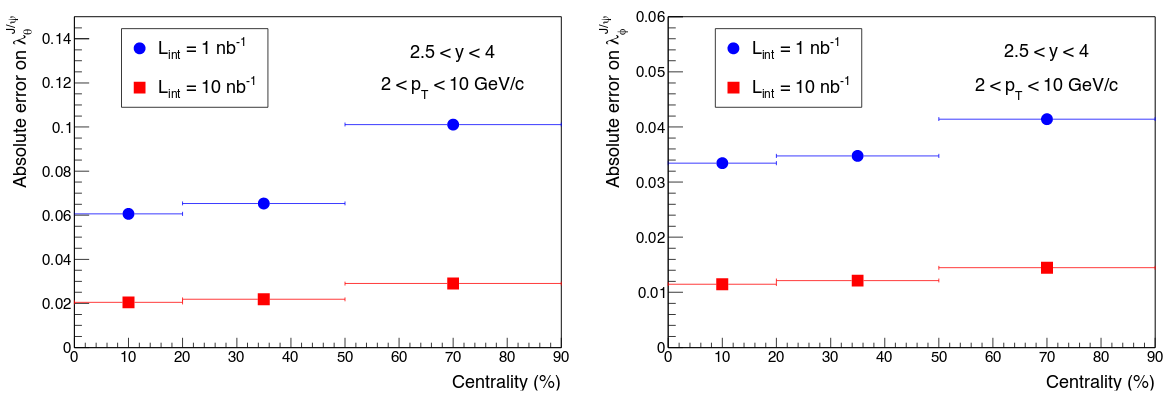
\includegraphics[width=\textwidth]{fig/alice/jpsi_polarisation.png}
\end{center}

 \caption{prompt J/psi polarisation~\cite{Abelev:1475243}}
\end{figure}

\begin{figure}
\begin{center}
 ?
\end{center}

 \caption{prompt psi(2S) RAA (and yields) vs. Npart (pT integrated) }
\end{figure}

\begin{figure}
\begin{center}
 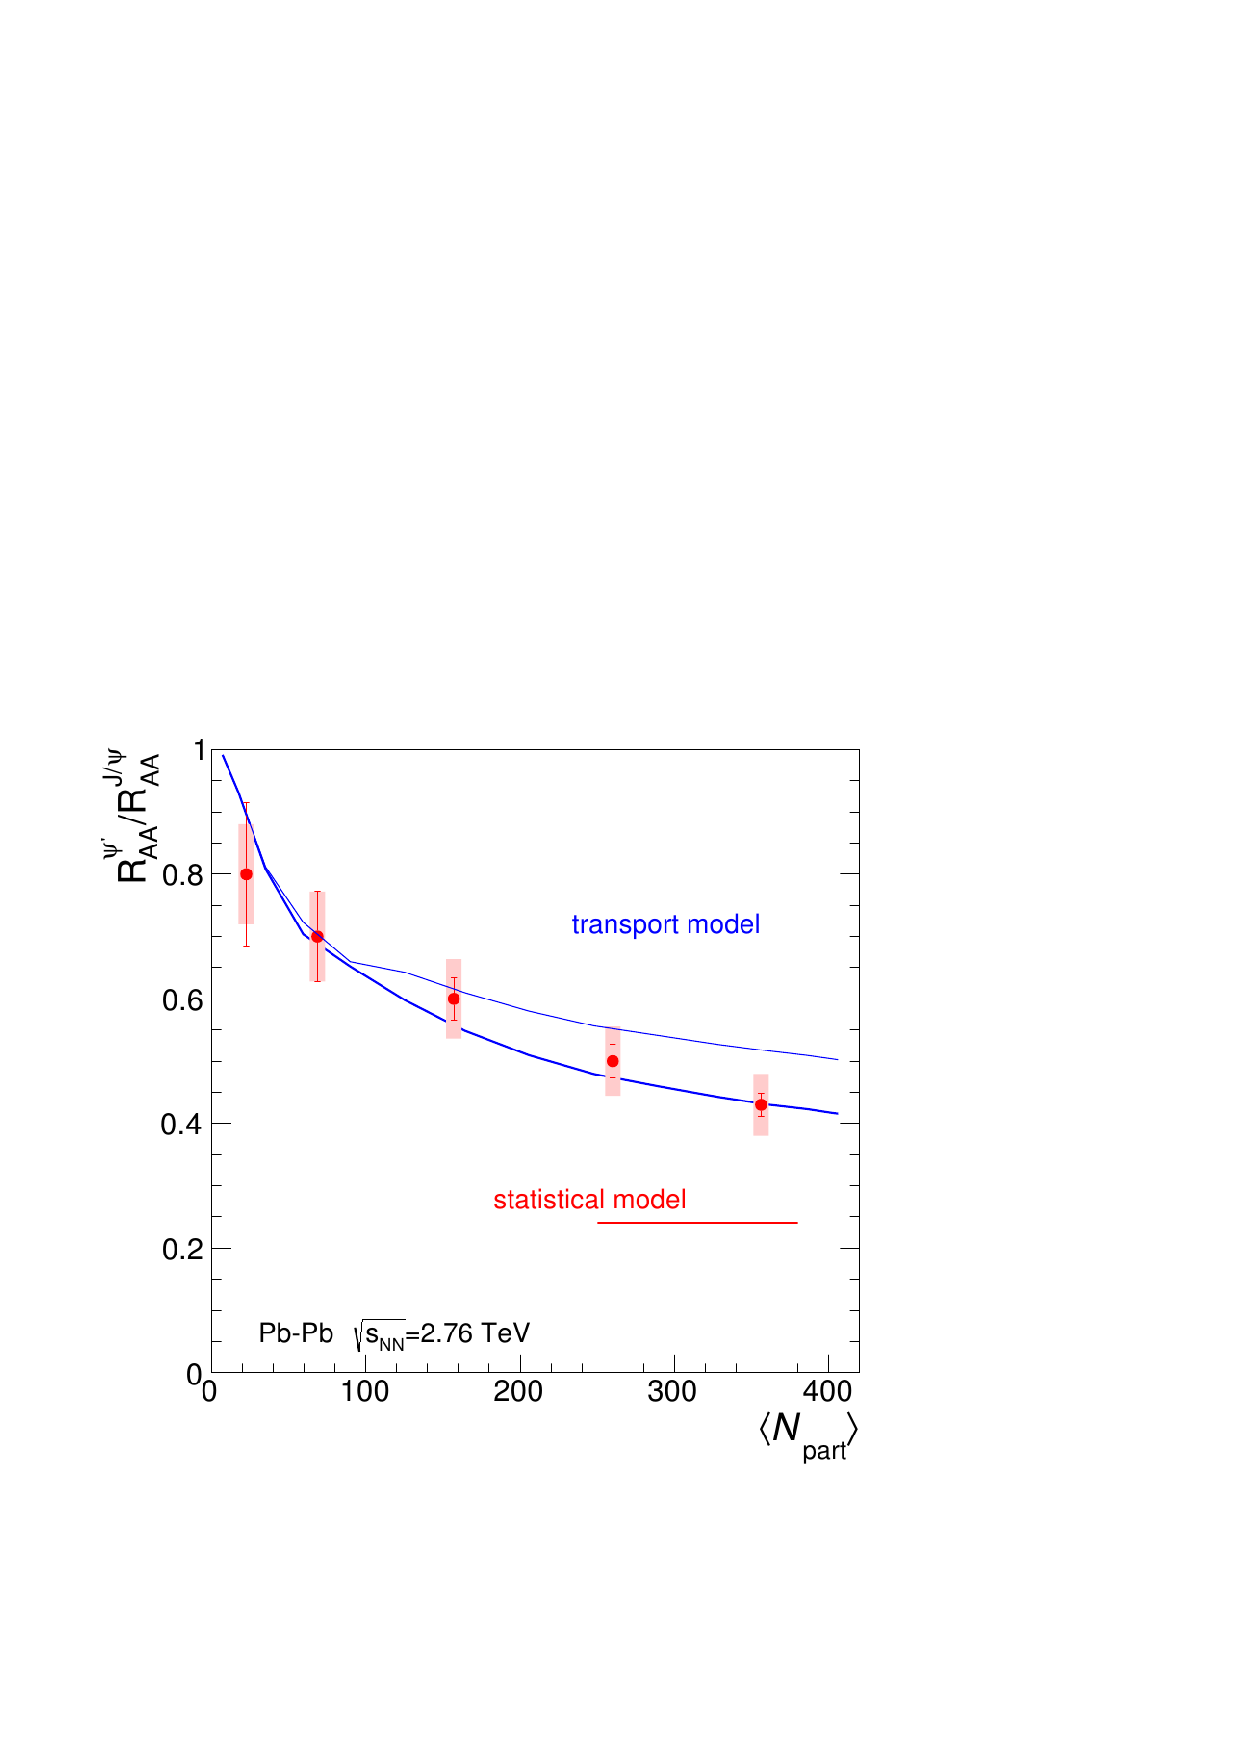
\includegraphics[width=0.32\textwidth]{fig/alice/alice_dr_psi_projected}
 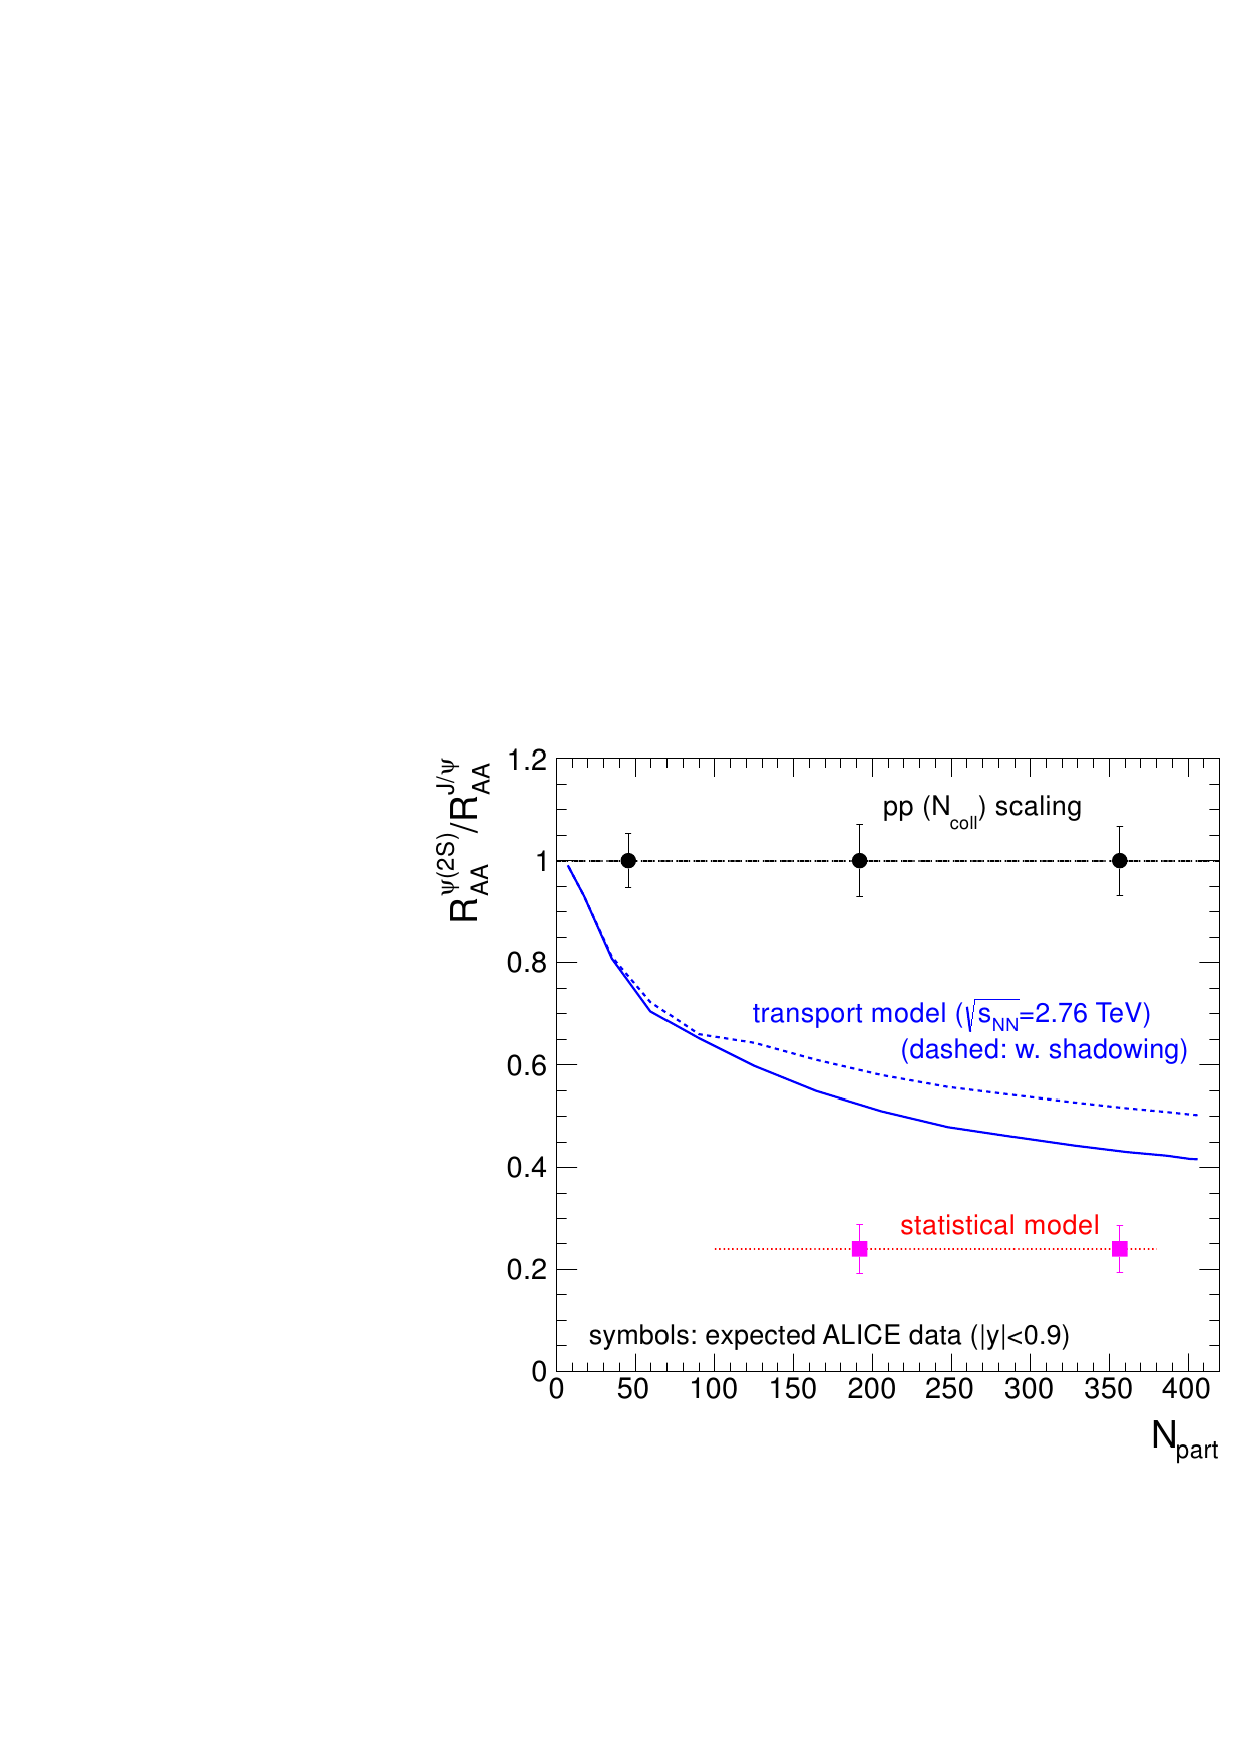
\includegraphics[width=0.32\textwidth]{fig/alice/alice_dr_psi_projected2}
\end{center}

 \caption{prompt psi(2S)/J/psi (or psi2S RAA) vs. Npart: $|y|<0.9 (2.4)$, $2.5<|y|<4$}
\end{figure}

\begin{figure}
\begin{center}
 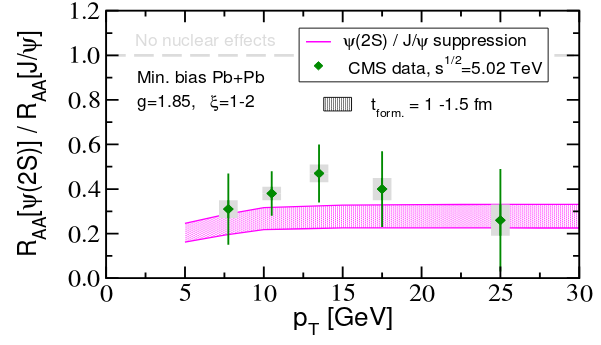
\includegraphics[width=0.32\textwidth]{fig/theory/psi_dr_vitev.png}
\end{center}

 \caption{prompt psi(2S) (and J/psi, or ratio) vs. pT (at low and high pT) }
\end{figure}

\begin{figure}
...

 \caption{prompt psi(2S) v2 vs pT for 30--50\%}
\end{figure}

\begin{figure}
\begin{center}
 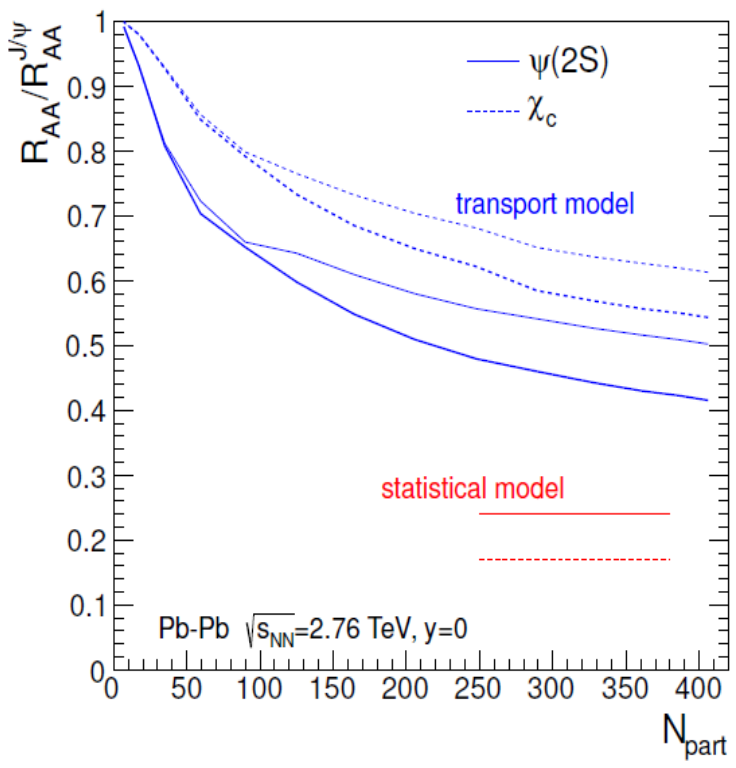
\includegraphics[width=0.32\textwidth]{fig/theory/chic.png}
\end{center}

 \caption{RAA of chic(1P), X(3872) vs pT for $|y|<2.4$}
\end{figure}



\subsection{Bottomonia in PbPb collisions (Main contributor: Emilien Chapon)}

\begin{figure}
\begin{center}
 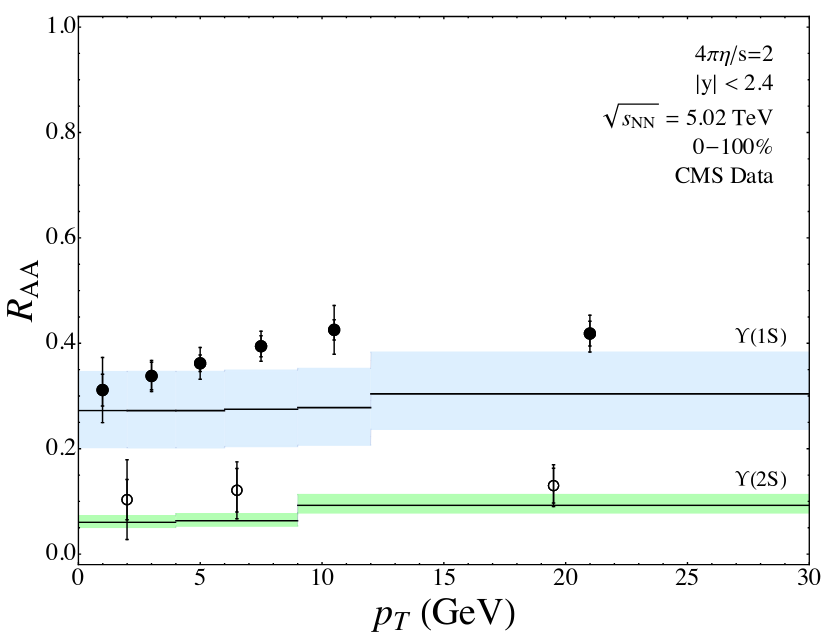
\includegraphics[width=0.32\textwidth]{fig/theory/strickland_pt.png}
 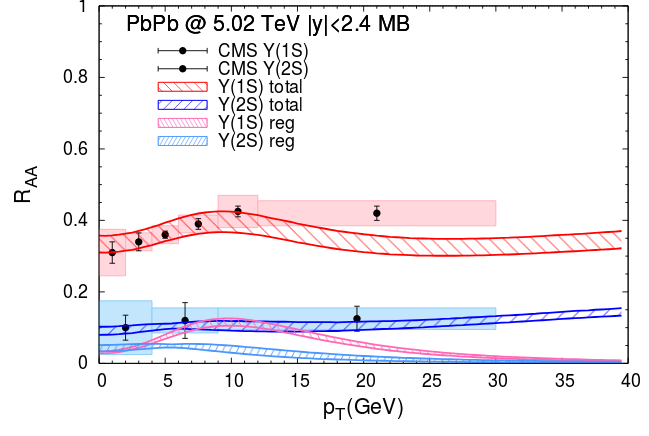
\includegraphics[width=0.32\textwidth]{fig/theory/rapp_raa_pt_CMS.png}
 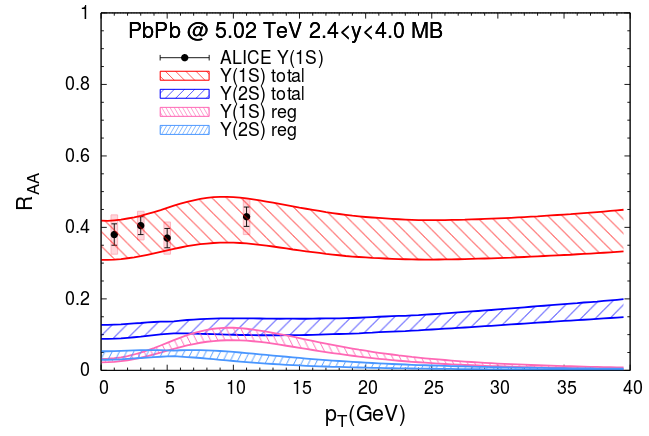
\includegraphics[width=0.32\textwidth]{fig/theory/rapp_raa_pt_ALICE.png}
 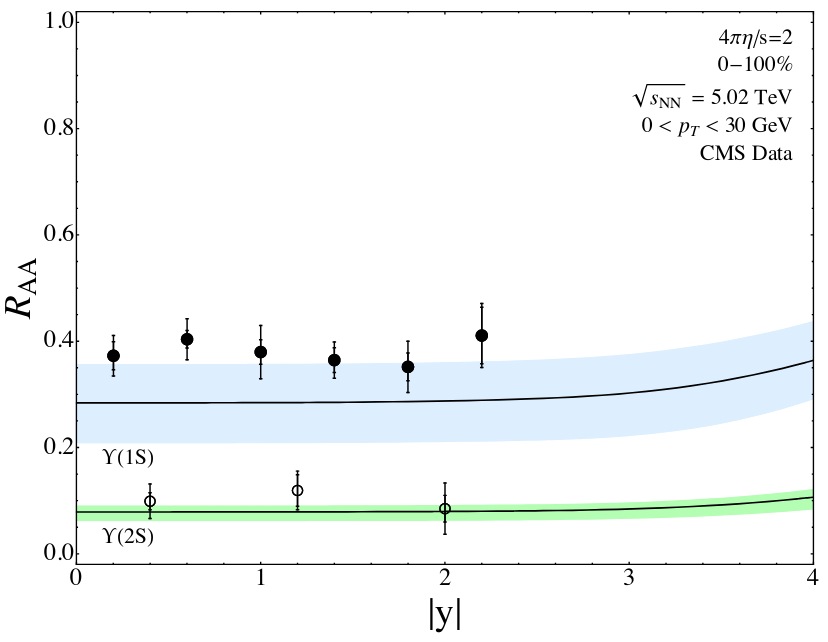
\includegraphics[width=0.32\textwidth]{fig/theory/strickland_rap.png}
\end{center}

 \caption{RAA (and yields?) vs pT, RAA vs y for 0--10\%, 0--100\%~\cite{Krouppa:2017jlg,Du:2017qkv} }
\end{figure}

\begin{figure}
\begin{center}
 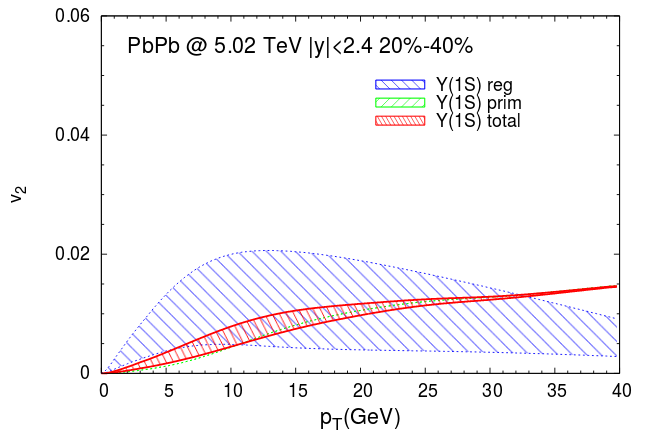
\includegraphics[width=0.32\textwidth]{fig/theory/rapp_v2_1S.png}
 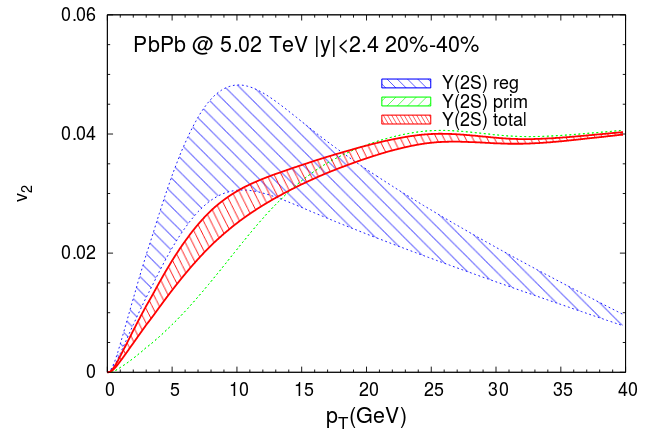
\includegraphics[width=0.32\textwidth]{fig/theory/rapp_v2_2S.png}
\end{center}

 \caption{v2 vs pT 30--50\%~\cite{Du:2017qkv}}
\end{figure}

\begin{figure}
\begin{center}
 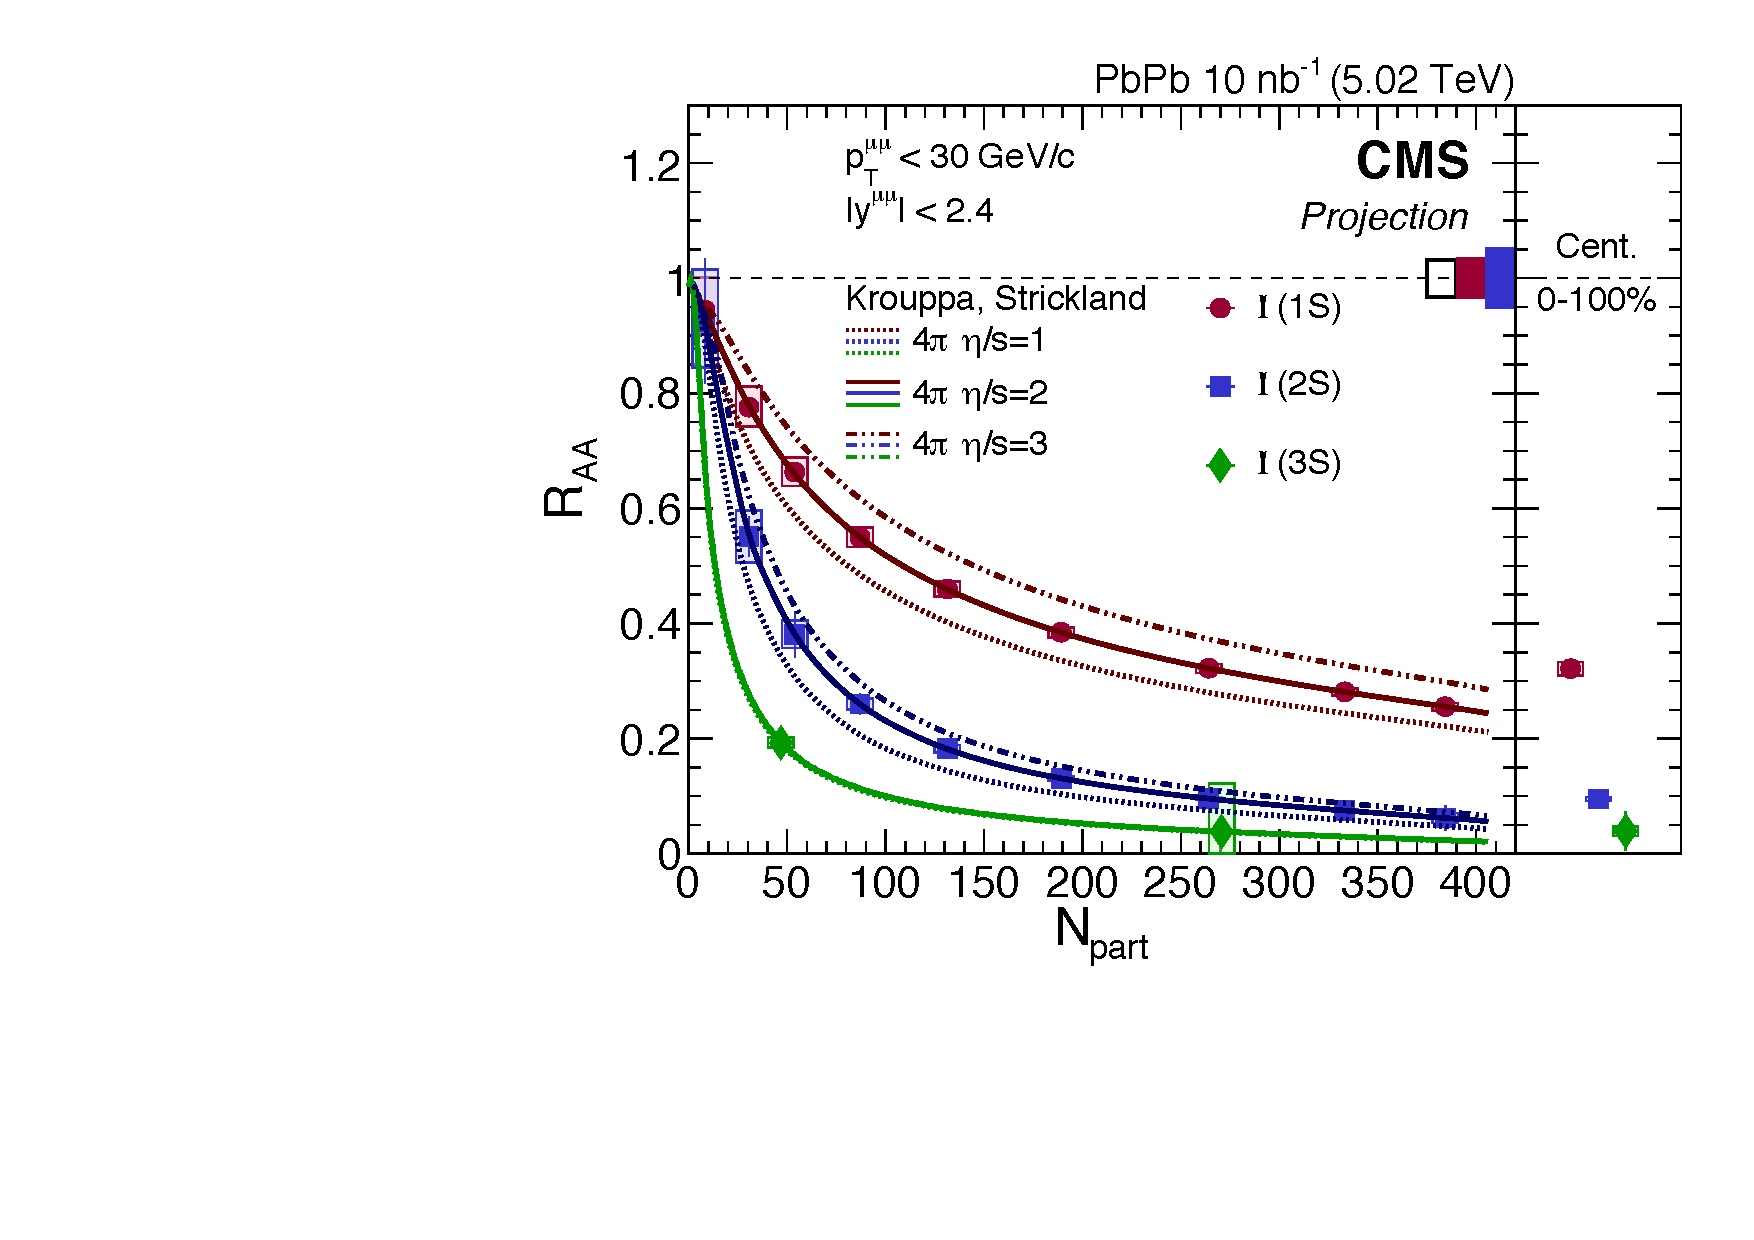
\includegraphics[width=0.32\textwidth]{fig/cms/CMS-PAS-FTR-17-002_Figure_008-b.pdf}
 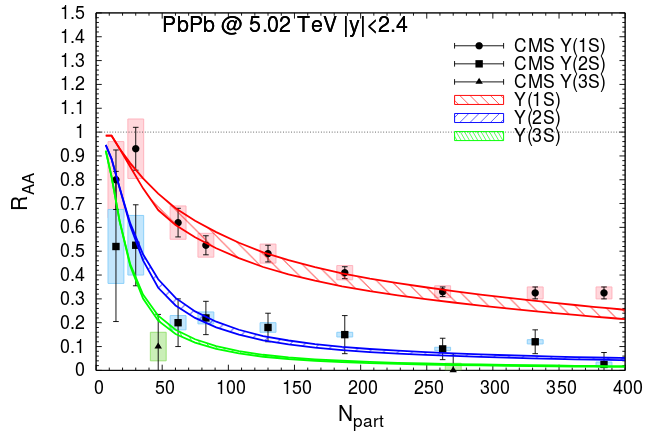
\includegraphics[width=0.32\textwidth]{fig/theory/rapp_raa_npart_CMS.png}
 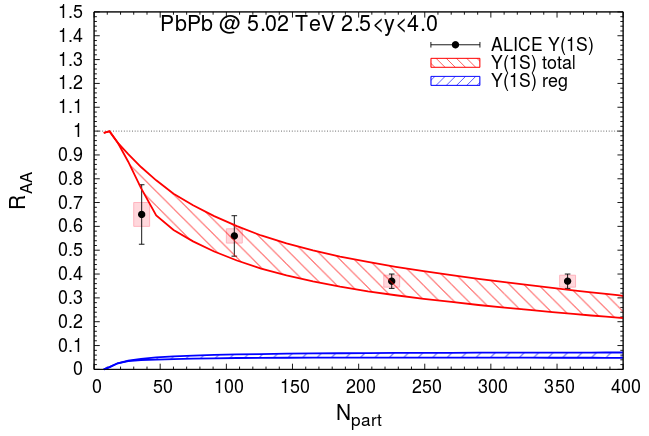
\includegraphics[width=0.32\textwidth]{fig/theory/rapp_raa_npart_ALICE.png}
\end{center}

 \caption{Y(1S,2S,3S) RAA vs Npart\cite{CMS-PAS-FTR-17-002,Krouppa:2016jcl,Du:2017qkv}}
\end{figure}

\begin{figure}
 \begin{center}
  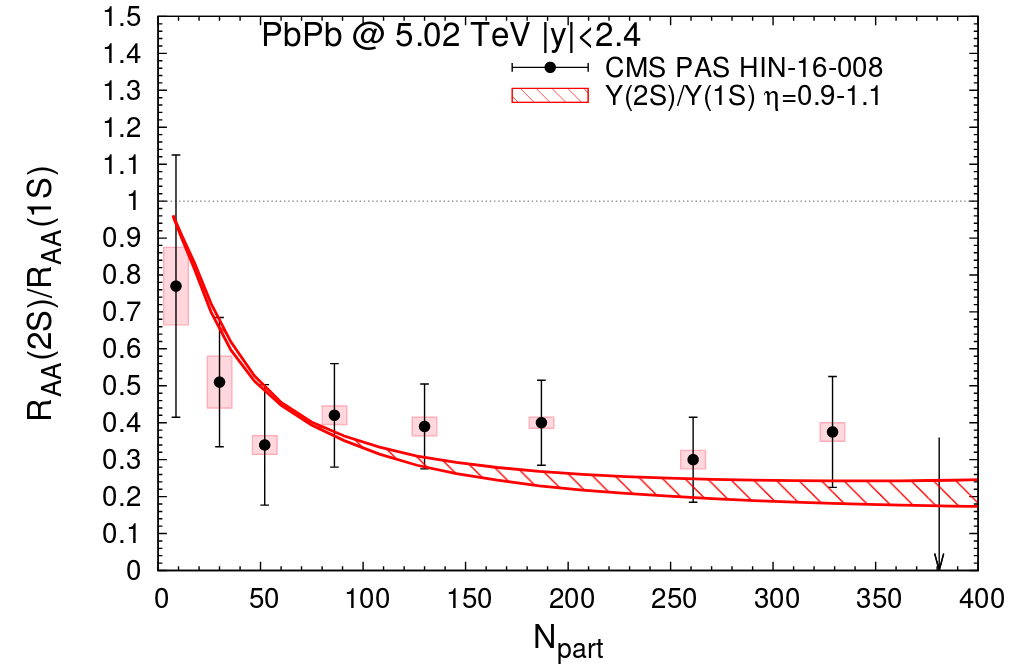
\includegraphics[width=0.32\textwidth]{fig/theory/rapp_dr_npart.png}
 \end{center}

 \caption{Y(2S,3S)/Y(1S) vs Npart~\cite{Du:2017qkv}}
\end{figure}


Also a figure on the prospects for the $B_c$ meson?

\subsection{Quarkonia in pp and pPb collisions}

\begin{figure}
 \begin{center}
  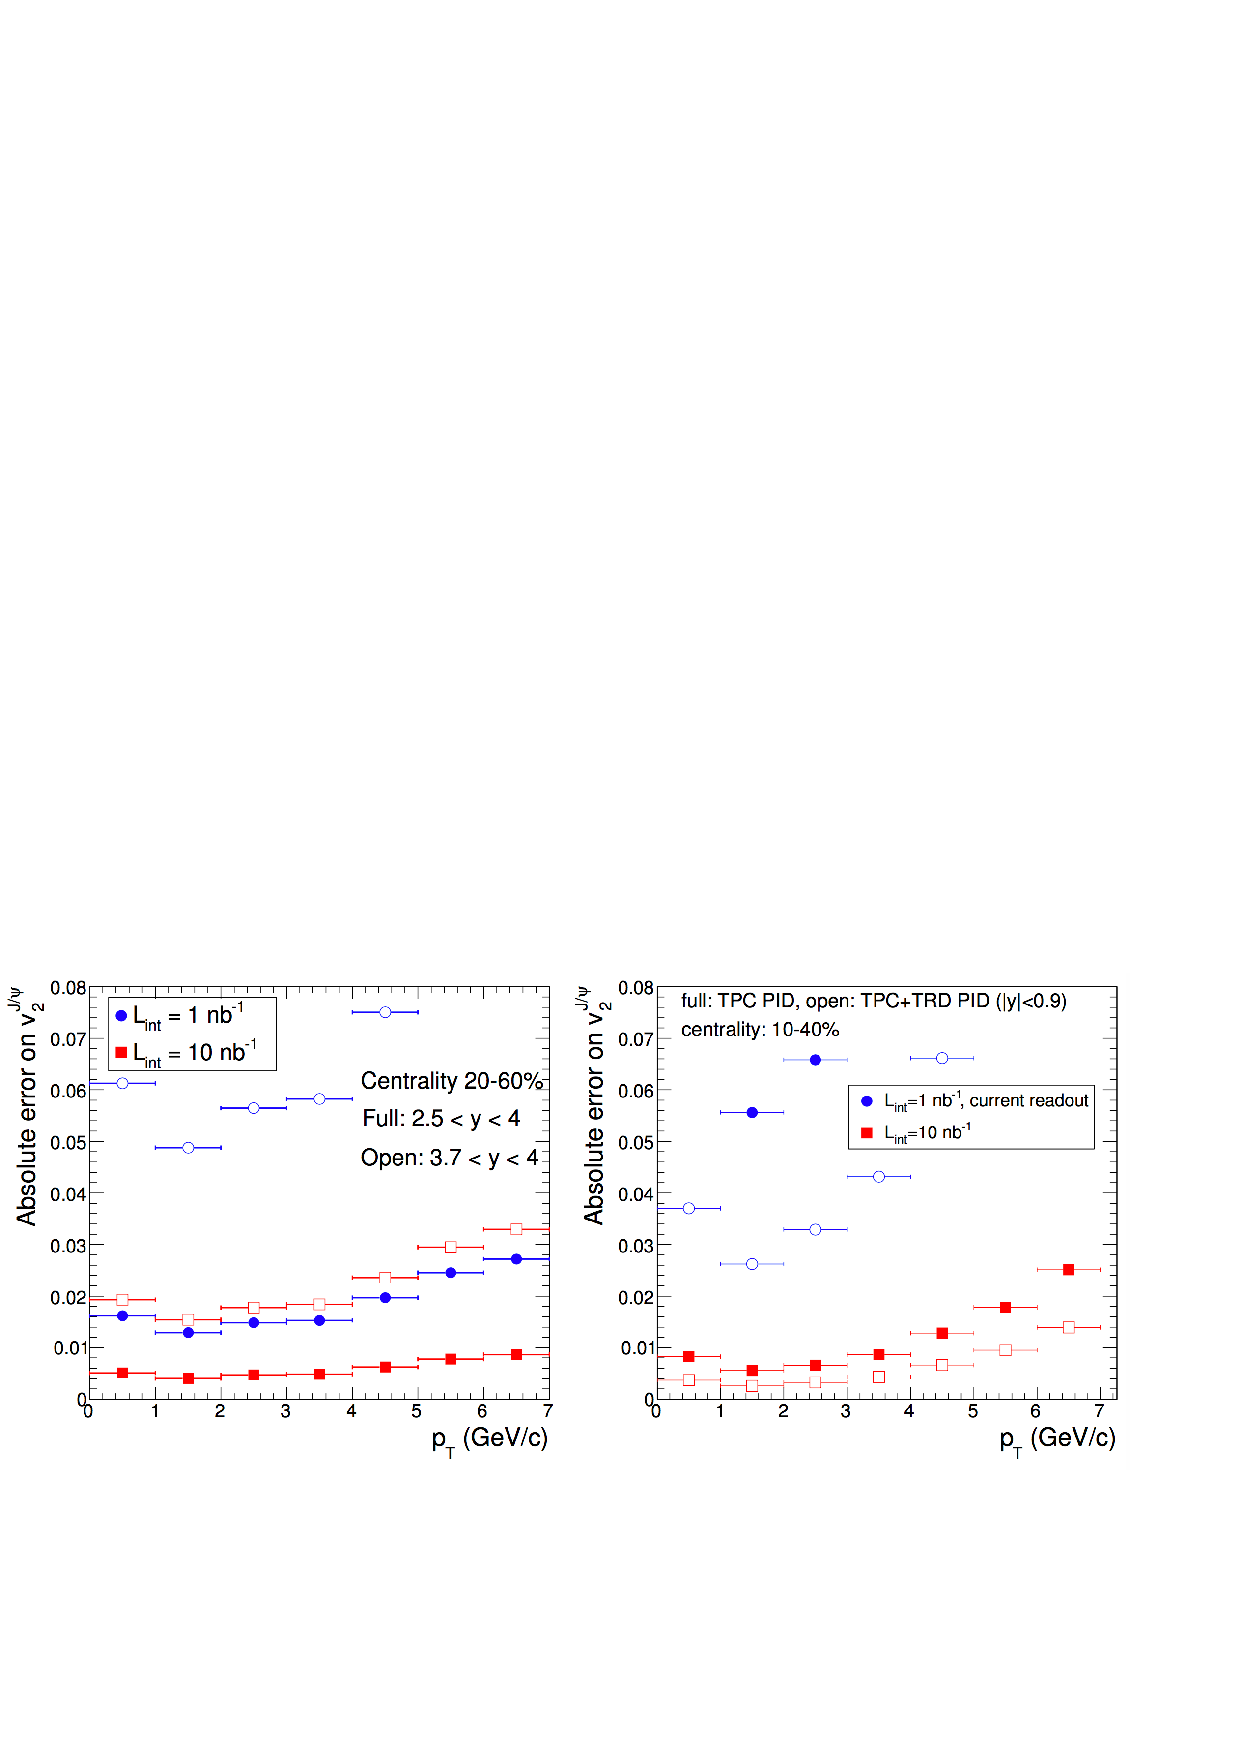
\includegraphics[width=0.32\textwidth]{fig/alice/alice_jpsi_v2_projected.pdf}
  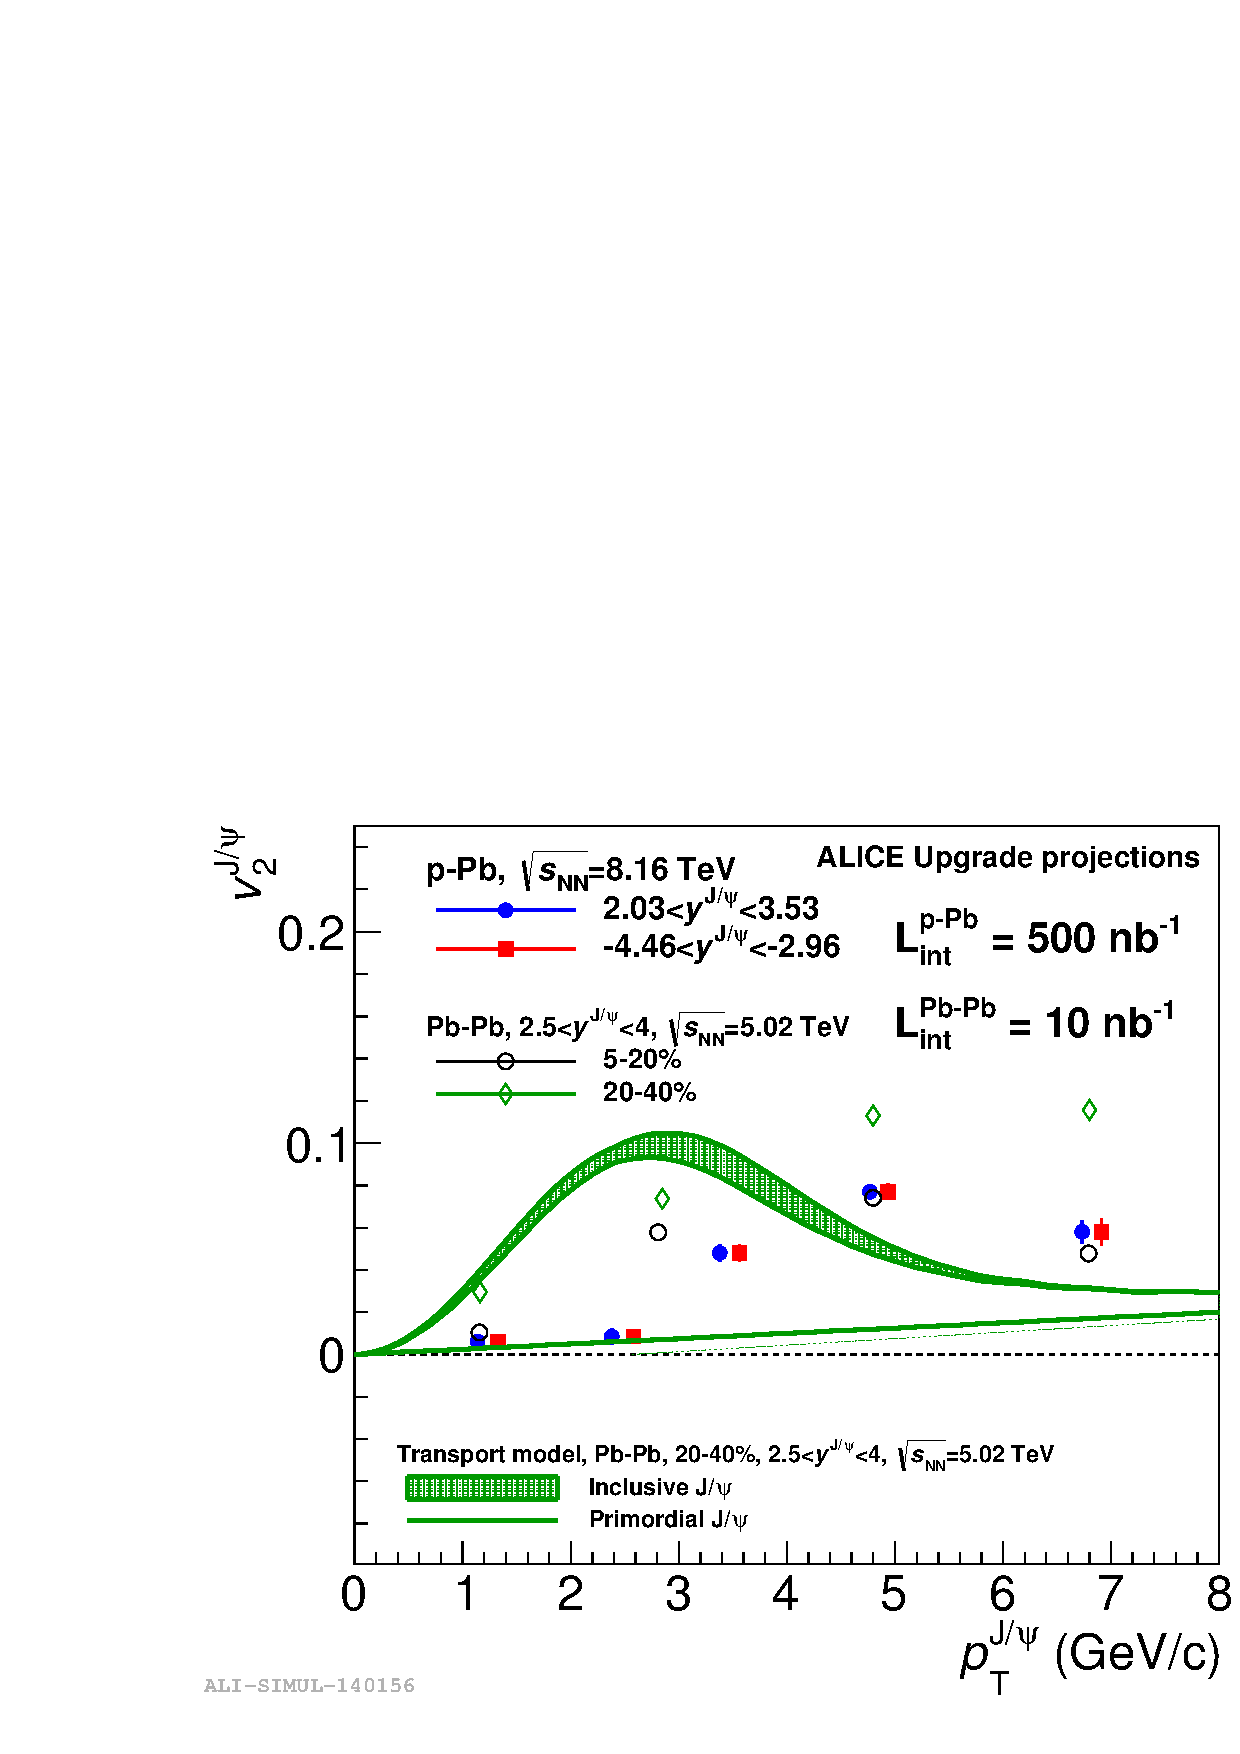
\includegraphics[width=0.32\textwidth]{fig/alice/alice_jpsi_v2_projected2.pdf}
 \end{center}

 \caption{prompt J/psi v2 and v3 (separately for negative and positive $y_{CM}$)}
\end{figure}

\begin{figure}
 \begin{center}
  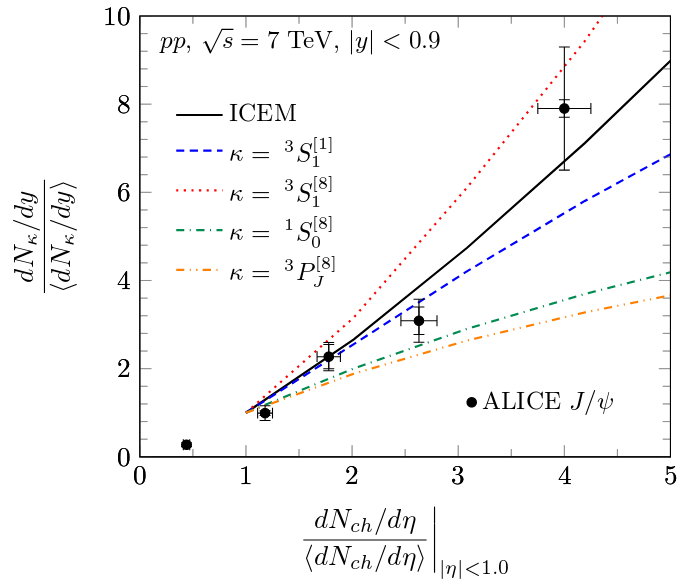
\includegraphics[width=0.5\textwidth]{fig/theory/cgc_jpsi_nch.png}
 \end{center}

 \caption{prompt J/psi vs Nch (also in pp)~\cite{Ma:2018bax}}
\end{figure}

\begin{figure}
 \begin{center}
 theory curves here
 \end{center}

 \caption{RpA vs pT for excited states: psi(2S), upsilon(2S,3S), chic(1P) (separately for negative and positive $y_{CM}$)}
\end{figure}

To be also discussed: SMOG results from LHCb.



\bibliographystyle{report}
\bibliography{bib/section}

\end{document}
